\chapter*{Measuring the output voltage of RME FIREFACE UCX}
A test was made to get a view of the output voltage of the sound card and its corresponding digital value. The test will be done with a continues \SI{1}{\kilo\hertz} tone, because the all measurement will be done with calibrated sound card and in the area of the amplifier, where the transfer function is linear.

\section*{Materials and setup}
To measure the output voltage, the following materials are used:
\begin{itemize}
\item Digilent Analog Discovery 2 (Oscilloscope)
\begin{itemize}[noitemsep]
\item AAU-number: 2179-12
\item Serial number: DA3716C
\end{itemize}
\item RME FIREFACE ucx (Soundcard)
\begin{itemize}[noitemsep]
\item AAU-number: 108230
\item Serial number: 23811948
\end{itemize}
\item Digilent Waveforms 2015 (PC - software)
\item MATLAB 2017b (PC - software)
\item SynchronizedPlaybackAcquirer, where playgain is the output attenuation in \si{\decibel} (Made by MATLAB)
\end{itemize}

\begin{figure}[htbp!]
\centering
\begin{picture}(0,0)%
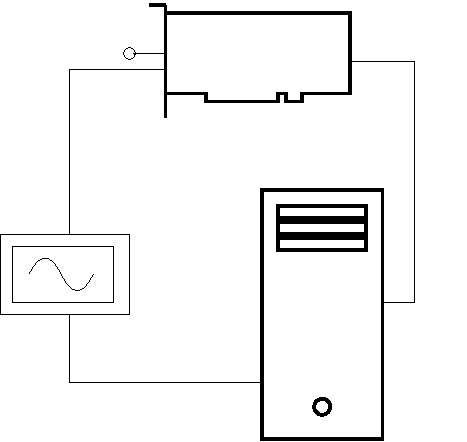
\includegraphics{RME_voltage_out.pdf}%
\end{picture}%
\setlength{\unitlength}{2818sp}%
%
\begingroup\makeatletter\ifx\SetFigFont\undefined%
\gdef\SetFigFont#1#2#3#4#5{%
  \reset@font\fontsize{#1}{#2pt}%
  \fontfamily{#3}\fontseries{#4}\fontshape{#5}%
  \selectfont}%
\fi\endgroup%
\begin{picture}(5212,4926)(6964,-7474)
\put(10036,-6361){Computer}%
\put(9271,-3211){Sound Card}%
\put(8171,-2996){In}%
\put(8171,-3526){Out}%
\put(7831,-5056){In}%
\put(5431,-5856){Oscilloscope}%
\put(8236,-6676){USB}%
\put(11746,-4606){USB}%
\end{picture}%
\caption{Setup for measuring output voltage of the sound card.}
		\label{fig:appendix:rme_output_voltage}
\end{figure}

\section*{Test procedure}


\begin{enumerate}
\item The materials are set up as in \autoref{fig:appendix:rme_output_voltage}.
\item A sinusoid with a frequency of \SI{1}{\kilo\hertz} and a digital amplitude of 1 is created.  
\item The sinusoid is played continuously at the output of the sound card with a playgain of  \SI{0}{\decibel}.
\item  A measurement of the sinusoid on the output of the sound card is made with Digilent Analog Discovery 2.
\item The data from Digilent Analog Discovery 2 is imported to MATLAB and plotted with the sinusoid created in MATLAB
\end{enumerate}

\section*{Results}

\begin{figure}[htbp!]
	\centering
		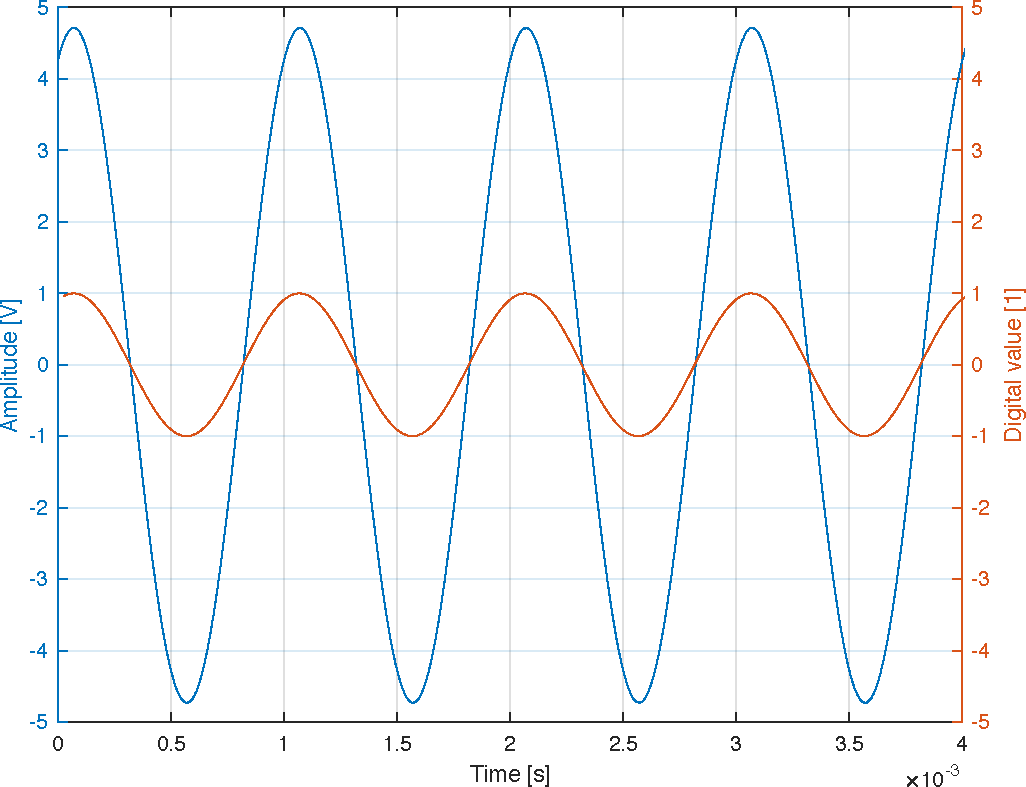
\includegraphics[width=1\textwidth]{rme_output_voltage.pdf}
		\caption{The output voltage compare to the digital value in MATLAB}
		\label{fig:appendix:rme_output_voltage_result}
\end{figure}

On  \autoref{fig:appendix:rme_output_voltage_result} it is seen that the digital number 1 in MATLAB corresponding to a voltage of \SI{4.7}{\volt} when the playgain is at \SI{0}{\decibel}. 

\section*{Conclusion}
It can be concluded that the factor between the digital number in MATLAB and the output voltage is 4.7 with playgain of \SI{0}{\decibel}. Since the sound card will be calibrated for every measurement, it is concluded that this factor is linear from \SI{20}{\hertz} to \SI{20}{\kilo\hertz}. 



